\documentclass{article}

% Document extensibility %
%
% Disables native paragraph indentation
\usepackage{parskip} 
%
% Provides further bullet options for lists
\usepackage{enumitem}

% Mathematical symbol and statement packages %
%
% Necessary
\usepackage{amsmath}
\usepackage{amssymb}
%
% Extensive fraction notation
\usepackage{xfrac}
%
% Generic mathematical commands
% Notable: \degree, \celcius
\usepackage{gensymb}
%
% Variable vector notation (arrow above variable)
\usepackage{esvect}
%
% Multiline boxed equations
\usepackage{empheq}
%
% SI Unit
\usepackage{siunitx}
%
% More intuitive arrays/matrices
\usepackage{array}

% Graphic packages %
%
% Diagrams and illustrations
\usepackage{tikz}
\usetikzlibrary{positioning}
%
% Image insertion
\usepackage{graphicx}
\graphicspath{ {./} }

% Document content %
%
% Change title of table of contents
% \renewcommand{\contentsname}{Title}

\begin{document}

% Command `\hr` to insert horizontal rules
\newcommand{\hr}{\par\noindent\rule{\textwidth}{0.4pt}}

% Command to box and center math equations
\newcommand{\bc}[1]{
	\begin{equation*}
		\begin{boxed}
			{#1}
		\end{boxed}
	\end{equation*}
}

% Command for single line equations with a condition
\newcommand{\cond}[2]{
	\ifmmode
		{#1} \quad {#2}
	\else
		$$ {#1} \quad {#2} $$
	\fi
}

\tableofcontents

\section{Energy}

\begin{equation}
	KE = \frac{1}{2}mv^2
\end{equation}
\begin{equation}
	W = \Delta KE
\end{equation}

When you do work against a conservative force (gravity, springs, electro magnetism (1C)) that energy is stored by the force and can be released later.

If energy is conserved the change in \underline{total} energy for a given process is \underline{\underline{zero}}!

\subsection{Conservation of Energy}

\begin{equation}
	E_i = E_f
\end{equation}
\begin{equation}
	KE_i + PE_i = KE_f + PE_f
\end{equation}
If dealing only in gravity:
\begin{equation}
	\frac{1}{2}mv_i^2 + mgh_i = \frac{1}{2}mv_f^2 + mgh_f
\end{equation}

\subsection{Example - Energy}

\begin{enumerate}[label=\textbf{Step \arabic*:}]
	\item
		Sketch that includes:
		\begin{itemize}
			\item every position
			\item every speed
			\item index
			\item zero potential energy
		\end{itemize}
\end{enumerate}

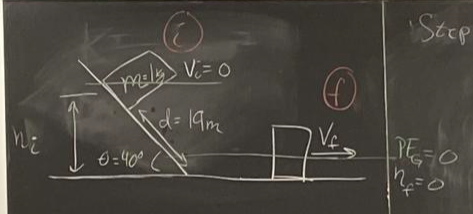
\includegraphics[width = \linewidth]{image.png}
\begin{align*}
	m & = \SI{1}{\kilogram} \\
	d & = \SI{19}{\meter} \\
	\theta & = \SI{40}{\degree} \\
	v_i & = 0 \\
	h_i & = ? \\
	v_f & = ? \\
	PE_G & = 0 \\
	h_f & = 0
\end{align*}
\begin{align*}
	\frac{1}{2}mv_i^2 + mgh_i & = \frac{1}{2}mv_f^2 + mgh_f \\
	\frac{1}{2}m(0) + mgh_i & = \frac{1}{2}mv_f^2 + mg(0) \\
	gh_i & = \frac{1}{2}v_f^2 \\
	v_f & = \sqrt{2gh_i} \\
	v_f & = \sqrt{2gd\sin(\theta)} \\
	v_f & = \sqrt{2(\SI{10}{\meter \per \second \squared})(\SI{19}{\meter})\sin(\SI{90}{\degree})} \\
	v_f & = \SI{15.6}{\meter \per \second}
\end{align*}

Supposed we do the experiment and we find $ v_f = \SI{11.6}{\meter \per \second} $. How much energy was lost to friction? How much energy was lost to friction? What is $ \mu $?
\begin{enumerate}[label=\textbf{\arabic*)}]
	\item
		Kinematics \\
		Find $ a, f, N \rightarrow f = \mu N $
	\item
		\begin{align*}
			W & = \Delta KE \\
			-fd & = \Delta KE
		\end{align*}
		find $ N \rightarrow f = \mu N $
\end{enumerate}
If you have a non-conservative force:
\begin{equation}
	E_i + W_{nc} = E_f
\end{equation}
\begin{tikzpicture}
	\node[circle, fill, inner sep = 1pt] (origin) {};
	\node (above_left) [above left = of origin] {$ f $};
	\node (above_right) [above right = of origin] {$ N $};
	\node (below) [below = of origin] {$ mg $};

	\foreach \node in {above_left, above_right, below}
		\draw[black, thick, ->] (origin) -- (\node);
\end{tikzpicture}
\begin{align*}
	\sum F_y & = 0 \\
	N & = mg\cos(\theta) \\
	f & = \mu mg\cos(\theta)
\end{align*}
\begin{align*}
	W_f & = -fd \\
	W_f & = -\mu mgd\cos(\theta)
\end{align*}
\begin{align*}
	E_i + W_f & = E_f \\
	mgd\sin(\theta) - \mu mgd\cos(\theta) & = \frac{1}{2}mv_f^2 \\
	gd\sin(\theta) - \mu gd\cos(\theta) & = \frac{1}{2}v_f^2 \\
	\mu & = \frac{2gd\sin(\theta) - v_f^2}{2gd\cos(\theta)}
\end{align*}

\subsection{Example - Pendulum}

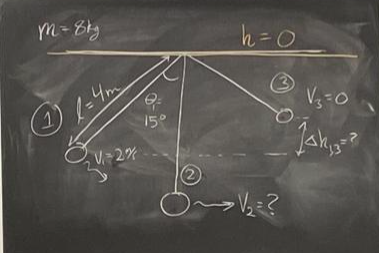
\includegraphics[width = \linewidth]{image_2.png}
\begin{align*}
	h_2 & = -\SI{4}{\meter} \\
	\cos(\theta_1) & = \frac{-h_1}{l} \\
	h_1 & = -l\cos(\theta_1) \\
	h_1 & = -(\SI{4}{\meter})\cos(\SI{15}{\degree}) \\
	h_1 & = \SI{-3.86}{\meter}
\end{align*}
\begin{align*}
	E_1 & = E_2 \\
	mgh_1 + \frac{1}{2}mv_1^2 & = mgh_2 + \frac{1}{2}mv_2^2 \\
	v_2^2 & = v_1^2 + 2g(h_1 - h_2) \\
	v_2 & = \sqrt{v_1^2 + 2g(h_1 - h_2)} \\
	v_2 & = \sqrt{(\SI{2}{\meter \per \second})^2 + 2(\SI{10}{\meter \per \second \squared})(-\SI{3.86}{\meter} - (-\SI{4}{\meter}))} \\
	v_2 & = \SI{2.6}{\meter \per \second}
\end{align*}
\begin{align*}
	E_1 & = E_3 \\
	mgh_1 + \frac{1}{2}mv_1^2 & = mgh_3 \\
	gh_1 + \frac{1}{2}v_1^2 & = gh_3 \\
	\frac{1}{2}v_1^2 & = g(h_3 - h_1) \\
	\Delta h_{1, 3} & = \frac{v_1^2}{2g} \\
	\Delta h_{1, 3} & = \frac{(\SI{2}{\meter \per \second})^2}{\SI{20}{\meter \per \second \squared}} \\
	\Delta h_{1, 3} & = \SI{0.2}{\meter}
\end{align*}

\section{Log Scale Graphs}

Log-log graph - x and y axes are log scale \\
Log scales are in sets of 10

\subsection{Power Law:}
\textbf{log-log}
\begin{align*}
	y = kx^n \\
	\log(y) & = \log(kx^n) \\
	\log(y) & = \log(k) + \log(x^n) \\
	\log(y) & = n \cdot \log(x) + \log(k) \\
	Y & = nX + K
\end{align*}
\textbf{semi log}
\begin{align*}
	y & = ae^{kx} \\
	\ln(y) & = \ln(ae^{kx}) \\
	\ln(y) & = \ln(a) + \ln(e^{kx}) \\
	\ln(y) & = \ln(a) + kx \\
	Y & = kx + \ln(a)
\end{align*}
\textbf{Slope}
\begin{align*}
	\text{Slope} & = \frac{\log(y_2) - \log(y_1)}{\log(x_2) - \log(x_1)}
\end{align*}

\end{document}
